%%%%%%%%%%%%%%%%%%%%%%%%%%%%%%%%%%%%%%%%%
% Short Sectioned Assignment
% L	aTeX Template
% Version 1.0 (5/5/12)
%
% This template has been downloaded from:
% http://www.LaTeXTemplates.com
%
% Original author:
% Frits Wenneker (http://www.howtotex.com)
%
% License:
% CC BY-NC-SA 3.0 (http://creativecommons.org/licenses/by-nc-sa/3.0/)
%
%%%%%%%%%%%%%%%%%%%%%%%%%%%%%%%%%%%%%%%%%

%----------------------------------------------------------------------------------------
%	PACKAGES AND OTHER DOCUMENT CONFIGURATIONS
%----------------------------------------------------------------------------------------

\documentclass[paper=a4, fontsize=11pt]{scrartcl} % A4 paper and 11pt font size
%\documentclass{article}
\usepackage{algorithm}
\usepackage{algpseudocode}
\usepackage{pifont}
\usepackage{listings}
\usepackage{multirow}
\usepackage{hyperref}
\usepackage[T1]{fontenc} % Use 8-bit encoding that has 256 glyphs
\usepackage{graphicx} % Required for including images
%\usepackage{fourier} % Use the Adobe Utopia font for the document - comment this line to return to the LaTeX default
\usepackage[english]{babel} % English language/hyphenation
\usepackage{amsmath,amsfonts,amsthm} % Math packages

\usepackage{setspace}
\doublespacing

\usepackage[margin=1in]{geometry}

\usepackage{indentfirst}

\usepackage{lipsum} % Used for inserting dummy 'Lorem ipsum' text into the template

\usepackage{sectsty} % Allows customizing section commands
\allsectionsfont{\centering \normalfont\scshape} % Make all sections centered, the default font and small caps

\usepackage{fancyhdr} % Custom headers and footers
\pagestyle{fancyplain} % Makes all pages in the document conform to the custom headers and footers
\fancyhead{} % No page header - if you want one, create it in the same way as the footers below
\fancyfoot[L]{} % Empty left footer
\fancyfoot[C]{} % Empty center footer
\fancyfoot[R]{\thepage} % Page numbering for right footer
\renewcommand{\headrulewidth}{0pt} % Remove header underlines
\renewcommand{\footrulewidth}{0pt} % Remove footer underlines
\setlength{\headheight}{13.6pt} % Customize the height of the header

\numberwithin{equation}{section} % Number equations within sections (i.e. 1.1, 1.2, 2.1, 2.2 instead of 1, 2, 3, 4)
\numberwithin{figure}{section} % Number figures within sections (i.e. 1.1, 1.2, 2.1, 2.2 instead of 1, 2, 3, 4)
\numberwithin{table}{section} % Number tables within sections (i.e. 1.1, 1.2, 2.1, 2.2 instead of 1, 2, 3, 4)

\setlength{\parindent}{1cm} % Removes all indentation from paragraphs - comment this line for an assignment with lots of text

%----------------------------------------------------------------------------------------
%	TITLE SECTION
%----------------------------------------------------------------------------------------

%\newcommand{\horrule}[1]{\rule{\linewidth}{#1}} % Create horizontal rule command with 1 argument of height

%\title{	
%\normalfont \normalsize 
%\textsc{Wayne State University, CS} \\ [25pt] % Your university, school and/or department name(s)
%\horrule{0.5pt} \\[0.4cm] % Thin top horizontal rule
%\huge Face Verification Problem on the Large Scale Datasets \\ % The assignment title
%\horrule{2pt} \\[0.5cm] % Thick bottom horizontal rule
%}

%\author{PhD student: Artem Komarichev} % Your name

%\textsc{Advisor: Prof. Xuewen Chen} \\ [25pt]

%\date{\normalsize\today} % Today's date or a custom date

\begin{document}

\begin{titlepage}
    \begin{center}
        \vspace*{1cm}
        \LARGE
        Literature Survey \\
        \vspace{0.5cm}
        \Huge
        \textbf{Face Verification Problem on \\ the Large Scale Datasets}
        
        \vspace{0.5cm}
        \LARGE
        %Thesis Subtitle
        
        \vspace{5.5cm}
        
        Ph.D. candidate: \textbf{Artem Komarichev}
        
        Research advisor: \textbf{Prof. Xue-wen Chen}
        
        \vfill
        
        
        \vspace{0.8cm}
        
        
\includegraphics[scale=0.15]{pictures/warrior_banded_logo.jpg}
        
        \Large
        Department of Computer Science\\
        Wayne State University\\
        USA\\
        
    \end{center}
\end{titlepage}

%\maketitle % Print the title

%----------------------------------------------------------------------------------------
%	PROBLEM 1
%----------------------------------------------------------------------------------------

\newpage

\section{Introduction}

In the recent few years the interest in face recognition problems was increased significantly. One of the reasons behind this that now we have more powerful machines than couple decades ago which we can use to run more complex models. Moreover with the rapid grough in the development of convolutional netural networks (CNN) and deep architectures we could learn much better feature representations to make our predictions more accurate. Plus, there are a plenty of potential areas where we can apply our models such as: biometrics, information security, law enforcement and surveillance, access control and many others \cite{zhao2003face}. \par
Face recognition can be divided into several directions:
\begin{itemize}
  \item face verification
  \item face identification
  \item face detection
  \item face clustering
\end{itemize}

The main goal of \textit{face verification} is to define whether two face images belong to the same person or not. \textit{Face detection} is basically defining are there faces in the image, and if it is true, just return their locations in this digital image \cite{yang2002detecting}. The goal of \textit{face identification} is to assign each image to appropriate class in a dabase \cite{seo2011face}. \textit{Face clustering} defines common people among all available face images in the database. I want to concentrate only on face verification problem in this literature survey. \par

What does make face recognition problem hard to be solved? Some: illumination, rotation, different poses, occlusion \cite{ekenel2009facial}, facial expressions and so on. One of the datasets which reflects these difficulties is PIE (pose, illumination, and expression) dataset \cite{sim2002cmu}. The examples of image pairs you can see in Fig. 1 (I will add image next time). And it was considered to be very difficult to solve until the guys from Google proposed their solution \cite{schroff2015facenet} and solved it.

The other issue which I would like to consider here is using of large-scale datasets in solving problem. In order to effectively run any face verfification model on huge dataset we most likely need to parallelize our solution. There is two possible ways to make this: model parallelization and data parallelization \cite{dean2012large}. I will cover them in more details later and show some state-of-the-art applications. \par

%Alongside with the development of deep conovolutional networks, the researchers %started to apply deep architectures in their models to solve face verification %problem. LDA, SVM was also applied (I need to find papers).\par 

I will also descibe two widely used datasets for evaluation: Labeled Faces in the Wild (LFW) and Youtube Faces DB (YTF).

\section{DeepFace}
Comparing different reduced architectures (1) without second conovolutional layer, 2) without first two locally connected layers, and 3) without three these layers) with the original one, they showed that the deep of the architecture is a critical issue. Deeper DNN can learn better feature representations. Therefore, deeper architectures shows higher final accuracy than shallower ones does. \par
In conclusion, they achieved the new state-of-the-art on the LFW and YTF datasets by the time when the paper was published; they proposed a new alignment techniques based on 3D modeling of the face images in the unconstrained settings; they came up with a new DNN architecture which was trained on their own huge dataset.

\section{FaceNet}

Google proposed the new idea \cite{schroff2015facenet} and showed how face verification problem could be solved on the large-scale dataset. Their solution actually could be applied to different problems such as: face verification, face recognition and clustering. The key idea of their approach that they use Euclidean embedding space to find the similarity or difference between faces. The architecture of their model is represented on Fig. ?.?

\begin{center}
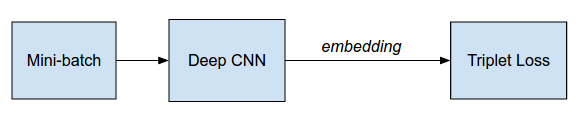
\includegraphics[scale=0.5]{pictures/arch_facenet.png}
\par\large\textit{Figure ?.?: FaceNet architecture.}
\end{center}

\subsection{Triplet Loss} 

Their most significant contribution is so-called "triplet loss". During the training process this loss minimizes the distances between similar faces and maximizes one between different faces.

Loss function that they were using was:
	\begin{align}
	\begin{split}
		 Loss = \sum_{j}^N \left( ||f(x_j^a)-f(x_j^p)||^2_2  - ||f(x_j^a)-f(x_j^n)||^2_2 + \gamma \right)
	\end{split}
	\end{align}
	
where $N$ is a possible set of all triplets in the dataset; $f(x)$ - embedding, that translates image $x$ into Euclidean space; $x_j^a$ - "anchor" image; $x_j^p$ - "positive" image, which should be close to an anchor image; $x_j^n$ - "negative" image; $\gamma$ - margin between positive and negative images.

We are interested in such triplets which violetes the following constraint $||f(x_j^a)-f(x_j^p)||^2_2 + \gamma < ||f(x_j^a)-f(x_j^n)||^2_2$. Only these triplets will contribute to our model during the training process. The only open question how to select such triplets.

They were selecting such pairs where distance between "anchor" and "positive" image was maximized ("hard positive") and the distance between "anchor" and "negative" was as small as possible ("hard negative"), but not zero. It is obviously tricky to look for such triplets in the whole dataset each iteration. Intead they used mini-batch approach to find these "hard positive" and "hard negative" pairs. The size of the batch in their experiments was equal to 1800 examplars.

The problem with selecting hard negatives that $L2$ distance could be equal to 0. Instead they were considering only the cases where the distance of hard positive and anchor less than the distance between hard negative and anchor. They called  them "semi-hard" examplars. 

\subsection{Deep Architectures}

They used two different deep architectures to extract features: 
\begin{itemize}
  \item "Convnet model" developed by D. Zeiler and B. Fergus \cite{zeiler2014visualizing} based on Krizhevsky architecture \cite{krizhevsky2012imagenet}. Model was exteneded by adding $1\times1$ convolutional layer before each standard convolutional layer. These $1\times1$ convolutional kernels were suggested by \cite{min2013nin}. Total number of layers were equal to 22. Number of parameters to train is 140M.
  \item The other model was inspired by "GoogLeNet" Inception convolutional neural network \cite{szegedy2014going}. Their model is almost the same except that they used $L_2$ pooling instead of maxpooling in inception layers. Total number of layers were equal to 16. Number of parameters to train is around 6.6M-7.5M.
\end{itemize}
 
Inception model could be run on the mobile devices because of the small number of parameters to be trained. \par
They used rectified linear units in both these models.

\subsection{Experiments and results}
First I would like to mention that the size of their training dataset is close to 200M faces with 8M identities \cite{schroff2015facenet}, as stated in Table \ref{}. It is the biggest training dataset which exists at this moment in industry. \par
During their experiments they found out that 128 dimension of embedding is good enough for face recognition tasks. It is even possible to use less dimension, 64 for example, without significant loss of accuracy. \par
Both deep architectures showed almost the same results. Except the fact that Inception model is a way better in terms of performance. \par
The most interesting part is how the size of training dataset affects accuracy prediction. They compared the following sizes: millions of images, tens of millions, and hundreds of millions. The most significant impovement was got on the training dataset with tens of millions of examplars. So in their experiments they showed that the question how large your training dataset is important. The larger dataset the more accurate model you will get. But to get all these results they have to run their model for almost 700 hours (~1 month).  \par

Speaking of the accuracy of their model on two academic dataset: LFW and Youtube Faces DB, they achieved current state-of-the-art results. See results in Table ~\ref{tab:table2}.

\begin{table}[!htb]
\centering
\begin{tabular}{|l|l|l|l|l|}
\hline
\multirow{2}{*}{} Models & \multicolumn{2}{l|}{Datasets} \\ \cline{2-3} 
                  &   LFW  &  Youtube Faces DB        \\ \hline
               FaceNet   &  $\textbf{99.63}\% \pm$0.15   &   $\textbf{95.12}\% \pm$0.39       \\ \hline
               DeepFace &  ...   &  ...       \\ \hline
               Parkhi's approach		& $\textbf{98.65}\%$	 & $\textbf{97.3}\%$ \\ \hline
               DeepID2 &  ...   &  ...       \\ \hline
               DeepID2+ &  ...   &  ...       \\ \hline
               DeepID3 &  ...   &  ...       \\ \hline
               ... & ... & ... \\ \hline
\end{tabular}
\caption{State-of-the-art in face verification.}
\label{tab:table2}
\end{table}

\section{Parkhi's deep face approach}

Inspired by papers \cite{taigman2014deepface, schroff2015facenet}, guys from University of Oxford decided to create their own comparably large face dataset \cite{parkhi2015deep}. And the main reason behind this that these huge datasets from Facebook and Google are not publically available. This newly collected dataset includes 2.6M images belonging to 2,622 unique identities. It is the biggest training dataset for face recognition in the academia at this moment. \par
Besides providing algorithm how to collect this new dataset, they also tested three different models on this dataset from \cite{simonyan2014very}. Using their pretrained model they achieved comparably good results on LFW and YTF to the current state-of-the-art.\par
In terms of face verification problem, they applied the same triplet loss as was suggested here \cite{schroff2015facenet}. For embedding function, was chosen affine projection on Euclidean space.

\subsection{Model architectures}

The architectures A, B and D are same as in \cite{simonyan2014very}. All these three models are same in terms of the type of layers which were used. But they are different in terms of depth. For example, A had 8 convolutional layers and 3 fully-connected (FC) layers. Number of conovlutional layers in B and D models were increased by 2 and 5 respectively. \par 
Input images in all these three models had a size of $224\times224$ pixels. \par
Speaking of the number of filters, they started from 64 and after each max-pooling ($2\times2; stride = 2$) they increased that number twice, until it reached 512. Max-pooling was not applied ater each convolutional layer only at specific places. \par
The main important part of these deep architectures is that very small convolutional kernels ($3\times3$) were used across all convolutional layers. By using these small filters they achieved two goals \cite{simonyan2014very}. First, they reduced the number of parameters that should to be trained. Second improvement they achieved could be extracted from the following fact. 5 by 5 filters, for example, can be represented by the stack of two $3\times3$ consecutive filters without pooling in between. $7\times7$ filters can be replaced by a stack of three $3\times3$ filters. This fact shows us that more disciminative decision function can be learned by replacing one non-linear rectifier units by several ones. \par
The Local Response Normalization (LCN) \cite{krizhevsky2012imagenet} was not used. Because it was shown that LCN does not give any significant improvements in terms of accuracy of their models.

\subsection{Experiments and results}

The evaluation was performed on LFW and YTF datasets, but as the training data they used images from their newly collected dataset. More importantly unique identities from benchmark datasets and new one are different.\par
During the training proces, models B and D used pretrained parameters of A one instead of starting from scratch. \par
They considred several aspects in their experiments on LFW dataset. I will only describe here three of them. First, they evaluated the deep of architectures and how it depends on the accuracy. The experiments showed that B model ($\textbf{97.27}\%$) gave a slight boost in accuracy over model A ($\textbf{96.70}\%$), but model D didn't improve results of model B it performed even worse by giving $\textbf{96.73}\%$ of accuracy. And one of the potential reason for this, that the number of parameters are different. The other one that they used pre-trained parameters from A to train B and D models. By transfering pre-trained parameters one have to be careful with learning rate and momentum. Also they did not investigated random initialization in their experiments. Second, applying 2D allignment on the test dataset gave improvement in accuracy, but applying allignment to training dataset did not improve model. Third, by applying triplet loss they got $\textbf{99.13\%}$ accuracy. It is significant improvements over model B without embedding. \par
To sum it up, they used simpler architecture than was used in DeepID-2,2+,3 \cite{sun2014deep, sun2015deeply, sun2015deepid3} and their model was trained on the smaller dataset comparing to DeepFace and FaceNet approaches. Nevertheless, they achieved comparable results, see Table ~\ref{tab:table2}.
\newpage

\section{Conclusion}
The one drawback of all these large-scale approaches that they didn't use parallelization techniques explained earlier.

\newpage

\bibliographystyle{IEEEtranBST2/IEEEtran}

\bibliography{references}

\end{document}